


\tikzset{every picture/.style={line width=0.75pt}} %set default line width to 0.75pt        

\begin{tikzpicture}[x=0.75pt,y=0.75pt,yscale=-1,xscale=1]
%uncomment if require: \path (0,300); %set diagram left start at 0, and has height of 300

%Image [id:dp5400394261220618] 
\draw (345.17,143.14) node  {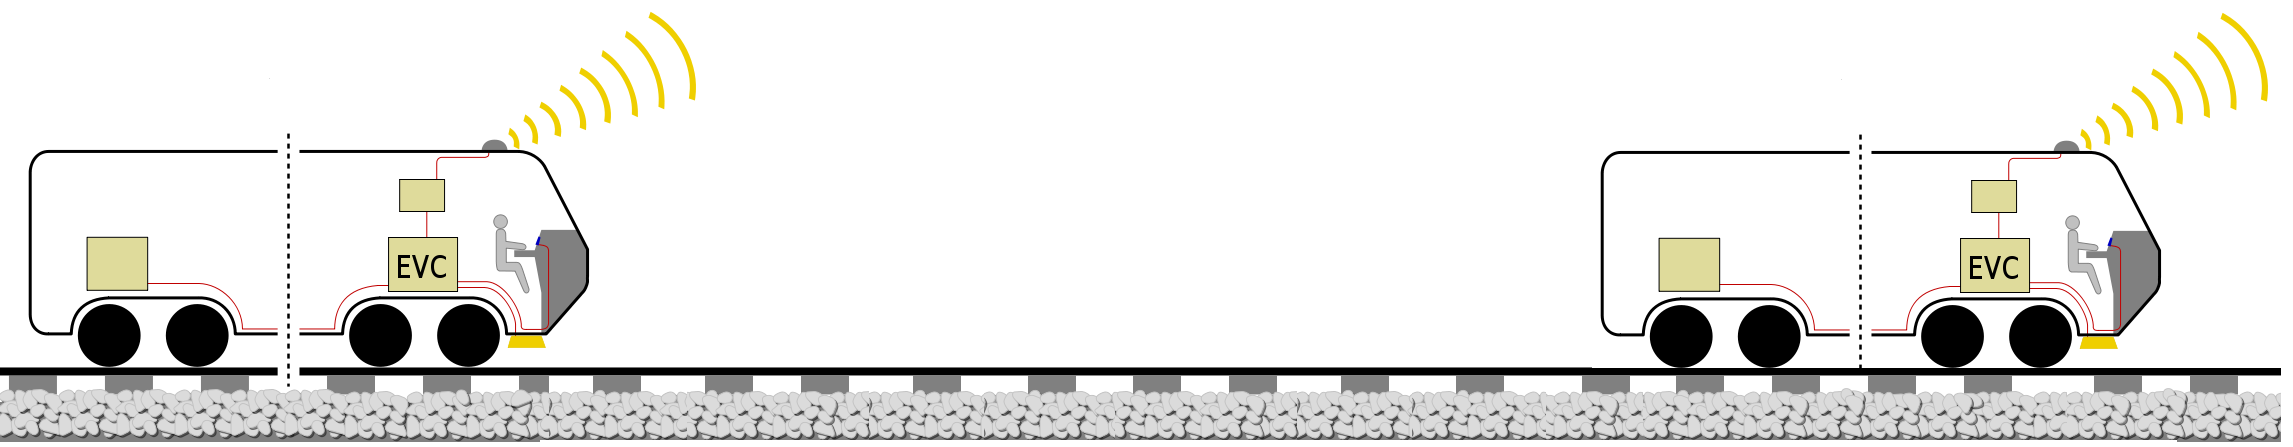
\includegraphics[width=451.25pt,height=87.97pt]{ERTMS_Background.png}};
%Straight Lines [id:da10086853571322152] 
\draw [line width=1.5]    (32,216) -- (641,215.01) ;
\draw [shift={(645,215)}, rotate = 179.91] [fill={rgb, 255:red, 0; green, 0; blue, 0 }  ][line width=0.08]  [draw opacity=0] (11.61,-5.58) -- (0,0) -- (11.61,5.58) -- cycle    ;
\draw [shift={(32,216)}, rotate = 179.91] [color={rgb, 255:red, 0; green, 0; blue, 0 }  ][line width=1.5]    (0,6.71) -- (0,-6.71)   ;
%Straight Lines [id:da4246282135374029] 
\draw    (397,172) -- (463,172) ;
\draw [shift={(463,172)}, rotate = 180] [color={rgb, 255:red, 0; green, 0; blue, 0 }  ][line width=0.75]    (0,5.59) -- (0,-5.59)   ;
\draw [shift={(397,172)}, rotate = 180] [color={rgb, 255:red, 0; green, 0; blue, 0 }  ][line width=0.75]    (0,5.59) -- (0,-5.59)   ;
%Straight Lines [id:da8337786703307539] 
\draw [color={rgb, 255:red, 245; green, 166; blue, 35 }  ,draw opacity=1 ][line width=1.5]    (33.71,94.62) -- (210,96) ;
%Straight Lines [id:da421538735336056] 
\draw    (200,170.75) -- (397,172) ;
\draw [shift={(397,172)}, rotate = 180.36] [color={rgb, 255:red, 0; green, 0; blue, 0 }  ][line width=0.75]    (0,5.59) -- (0,-5.59)   ;
\draw [shift={(200,170.75)}, rotate = 180.36] [color={rgb, 255:red, 0; green, 0; blue, 0 }  ][line width=0.75]    (0,5.59) -- (0,-5.59)   ;
%Straight Lines [id:da6915654353430236] 
\draw [color={rgb, 255:red, 74; green, 144; blue, 226 }  ,draw opacity=1 ][line width=1.5]    (397,74) -- (32.38,69.29) ;
%Straight Lines [id:da3836173430907017] 
\draw [color={rgb, 255:red, 74; green, 144; blue, 226 }  ,draw opacity=1 ][line width=1.5]    (397,74) -- (526,74) ;
%Curve Lines [id:da5699852019251703] 
\draw [color={rgb, 255:red, 245; green, 166; blue, 35 }  ,draw opacity=1 ][line width=1.5]    (210,96) .. controls (269.17,-78.92) and (309.67,84) .. (397,74) ;
%Shape: Circle [id:dp11642118006555191] 
\draw  [fill={rgb, 255:red, 0; green, 0; blue, 0 }  ,fill opacity=1 ] (392.42,73.91) .. controls (392.47,71.38) and (394.56,69.37) .. (397.09,69.42) .. controls (399.62,69.47) and (401.63,71.56) .. (401.58,74.09) .. controls (401.53,76.62) and (399.44,78.63) .. (396.91,78.58) .. controls (394.38,78.53) and (392.37,76.44) .. (392.42,73.91) -- cycle ;
%Straight Lines [id:da5295755202589745] 
\draw [line width=1.5]    (32,216) -- (32.98,10) ;
\draw [shift={(33,6)}, rotate = 90.27] [fill={rgb, 255:red, 0; green, 0; blue, 0 }  ][line width=0.08]  [draw opacity=0] (11.61,-5.58) -- (0,0) -- (11.61,5.58) -- cycle    ;
\draw [shift={(32,216)}, rotate = 90.27] [color={rgb, 255:red, 0; green, 0; blue, 0 }  ][line width=1.5]    (0,6.71) -- (0,-6.71)   ;
%Shape: Circle [id:dp011489270196951784] 
\draw  [fill={rgb, 255:red, 0; green, 0; blue, 0 }  ,fill opacity=1 ] (205.51,91.33) .. controls (205.56,88.79) and (207.65,86.78) .. (210.18,86.84) .. controls (212.71,86.89) and (214.73,88.98) .. (214.67,91.51) .. controls (214.62,94.04) and (212.53,96.05) .. (210,96) .. controls (207.47,95.95) and (205.46,93.86) .. (205.51,91.33) -- cycle ;
%Straight Lines [id:da9152914996132344] 
\draw  [dash pattern={on 4.5pt off 4.5pt}]  (199,152) -- (200.31,210.29) ;
\draw [shift={(200.38,213.29)}, rotate = 268.71] [fill={rgb, 255:red, 0; green, 0; blue, 0 }  ][line width=0.08]  [draw opacity=0] (8.93,-4.29) -- (0,0) -- (8.93,4.29) -- cycle    ;
%Straight Lines [id:da09482912953606859] 
\draw  [dash pattern={on 4.5pt off 4.5pt}]  (611,161) -- (612.3,208.95) ;
\draw [shift={(612.38,211.95)}, rotate = 268.45] [fill={rgb, 255:red, 0; green, 0; blue, 0 }  ][line width=0.08]  [draw opacity=0] (8.93,-4.29) -- (0,0) -- (8.93,4.29) -- cycle    ;
%Shape: Circle [id:dp5536555007859871] 
\draw  [fill={rgb, 255:red, 0; green, 0; blue, 0 }  ,fill opacity=1 ] (205.51,71.33) .. controls (205.56,68.79) and (207.65,66.78) .. (210.18,66.84) .. controls (212.71,66.89) and (214.73,68.98) .. (214.67,71.51) .. controls (214.62,74.04) and (212.53,76.05) .. (210,76) .. controls (207.47,75.95) and (205.46,73.86) .. (205.51,71.33) -- cycle ;

% Text Node
\draw (43,73.4) node [anchor=north west][inner sep=0.75pt]  [font=\normalsize]  {$v_{F}$};
% Text Node
\draw (190,220.4) node [anchor=north west][inner sep=0.75pt]  [font=\normalsize]  {$s_{F}(T_T)$};
% Text Node
\draw (590.5,217.4) node [anchor=north west][inner sep=0.75pt]  [font=\normalsize]  {$s_{L}(T_T)$};
% Text Node
\draw (417,146.9) node [anchor=north west][inner sep=0.75pt]  [font=\normalsize]  {$S_{L4}$};
% Text Node
\draw (43.33,47.07) node [anchor=north west][inner sep=0.75pt]  [font=\normalsize]  {$v_{L}$};
% Text Node
\draw (56,126.5) node [anchor=north west][inner sep=0.75pt]  [color={rgb, 255:red, 245; green, 166; blue, 35 }  ,opacity=1 ] [align=left] {Follower};
% Text Node
\draw (472,126.5) node [anchor=north west][inner sep=0.75pt]  [color={rgb, 255:red, 74; green, 144; blue, 226 }  ,opacity=1 ] [align=left] {Leader};
% Text Node
\draw (285.83,145.4) node [anchor=north west][inner sep=0.75pt]    {$d_{L3}(t_T)$};
% Text Node
\draw (247.67,23.73) node [anchor=north west][inner sep=0.75pt]    {$ \begin{array}{l}
\gamma^{F}\\
\end{array}$};
% Text Node
\draw (627.67,222.73) node [anchor=north west][inner sep=0.75pt]    {$t$};
% Text Node
\draw (14,15.07) node [anchor=north west][inner sep=0.75pt]    {$v$};
% Text Node
\draw (381.33,48.4) node [anchor=north west][inner sep=0.75pt]  [font=\normalsize]  {$V_{LoA}$};
% Text Node
\draw (180.33,75.07) node [anchor=north west][inner sep=0.75pt]  [font=\normalsize]  {$T_{T}$};
% Text Node
\draw (403.58,77.49) node [anchor=north west][inner sep=0.75pt]  [font=\normalsize]  {$T_{T} +T_{D}$};
% Text Node
\draw (17.33,218.07) node [anchor=north west][inner sep=0.75pt]  [font=\normalsize]  {$0$};
% Text Node
\draw (283.67,67.73) node [anchor=north west][inner sep=0.75pt]    {$ \begin{array}{l}
\gamma ^{L}\\
\end{array}$};


\end{tikzpicture}





